\documentclass[border=10pt]{standalone}
\usepackage[utf8]{inputenc}
\usepackage{pgfplots}
\pgfplotsset{compat=1.18}

% --- Colors ---
\definecolor{cCalcPC}{HTML}{4A90E2}   % Blue
\definecolor{cSendPC}{HTML}{F5A623}   % Orange
\definecolor{cCalcPSoC}{HTML}{7ED321} % Green
\definecolor{cSendPSoC}{HTML}{D0021B} % Red

\begin{document}
	
	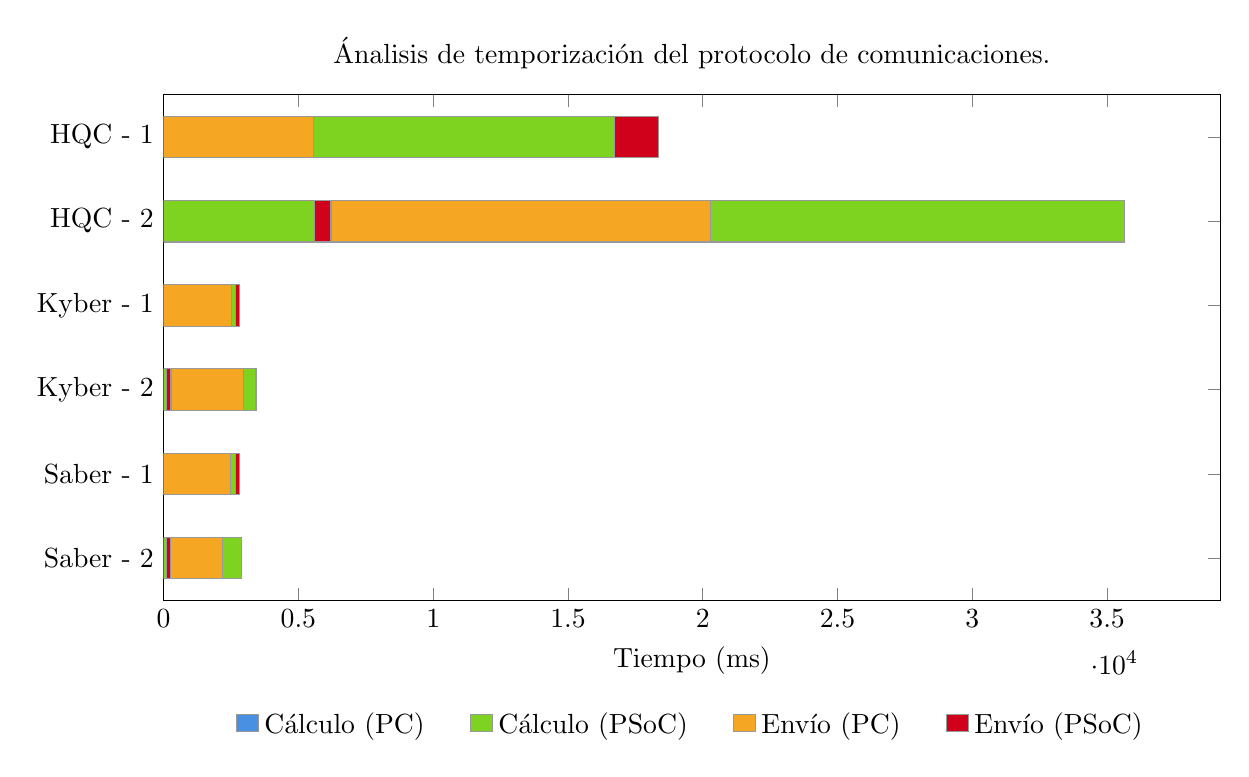
\begin{tikzpicture}
		\begin{axis}[
			xbar stacked,   % Horizontal stacked bars
			width=15cm, height=8cm,
			bar width=15pt,
			xmin=0,
			xlabel={Tiempo (ms)},
			title={Ánalisis de temporización del protocolo de comunicaciones.},
			% Y-Axis configuration
			ytick={0,1,2,3,4,5},
			yticklabels={HQC - 1, HQC - 2, Kyber - 1, Kyber - 2, Saber - 1, Saber - 2},
			y dir=reverse, % Keeps HQC-1 at the top
			% Legend configuration
			legend style={
				at={(0.5,-0.2)}, 
				anchor=north, 
				legend columns=-1, 
				draw=none,
				/tikz/every even column/.append style={column sep=0.5cm}
			},
			% No 'nodes near coords' means no numbers will be printed
			]
			
			% --- STEP 1 ---
			% Scenario 1 (Blue)
			\addplot[fill=cCalcPC, draw=black!40] coordinates { 
				(9.1,0) (0,1) (1.9,2) (0,3) (2.0,4) (0,5) 
			}; 
			\addlegendentry{Cálculo (PC)}
			
			% Scenario 2 (Green)
			\addplot[fill=cCalcPSoC, draw=black!40] coordinates { 
				(0,0) (5587,1) (0,2) (100,3) (0,4) (113,5) 
			}; 
			\addlegendentry{Cálculo (PSoC)}
			
			% --- STEP 2 ---
			% Scenario 1 (Orange)
			\addplot[fill=cSendPC, draw=black!40] coordinates { 
				(5541,0) (0,1) (2501,2) (0,3) (2466,4) (0,5) 
			}; 
			\addlegendentry{Envío (PC)}
			
			% Scenario 2 (Red)
			\addplot[fill=cSendPSoC, draw=black!40] coordinates { 
				(0,0) (614,1) (0,2) (176,3) (0,4) (147,5) 
			}; 
			\addlegendentry{Envío (PSoC)}
			
			% --- STEP 3 ---
			% Scenario 1 (Green)
			\addplot[fill=cCalcPSoC, draw=black!40, forget plot] coordinates { 
				(11177,0) (0,1) (150,2) (0,3) (194,4) (0,5) 
			}; 
			% Scenario 2 (Blue)
			\addplot[fill=cCalcPC, draw=black!40, forget plot] coordinates { 
				(0,0) (17.0,1) (0,2) (1.8,3) (0,4) (1.5,5) 
			}; 
			
			% --- STEP 4 ---
			% Scenario 1 (Red)
			\addplot[fill=cSendPSoC, draw=black!40, forget plot] coordinates { 
				(1620,0) (0,1) (176,2) (0,3) (165,4) (0,5) 
			}; 
			% Scenario 2 (Orange)
			\addplot[fill=cSendPC, draw=black!40, forget plot] coordinates { 
				(0,0) (14062,1) (0,2) (2687,3) (0,4) (1913,5) 
			}; 
			
			% --- STEP 5 ---
			% Scenario 1 (Blue)
			\addplot[fill=cCalcPC, draw=black!40, forget plot] coordinates { 
				(22.7,0) (0,1) (0.1,2) (0,3) (0.1,4) (0,5) 
			}; 
			% Scenario 2 (Green)
			\addplot[fill=cCalcPSoC, draw=black!40, forget plot] coordinates { 
				(0,0) (15350,1) (0,2) (464,3) (0,4) (725,5) 
			}; 
			
		\end{axis}
	\end{tikzpicture}
\end{document}